\documentclass{article}
\usepackage{tikz}
\usepackage{float}     % To force figure placement
\usepackage{siunitx}
\usepackage[T1]{fontenc}
\usepackage[utf8]{inputenc}
\usepackage{float}
\usepackage{xfrac} % For slanted fractions
\usepackage{graphicx}
\usepackage{amsmath}
\begin{document}
\section*{Woche 7 Aufgaben}
\subsection*{Question 1}
$\star$Auf dem Mond beträgt die Gravitationsfeldstärke nur ein Sechstel der Gravitationsfeldstärke auf der Erde. Ein Astronaut, dessen Gewicht auf der Erde 600~N beträgt, betritt die Mondoberfläche. Wie gross ist dort seine Masse?
\subsection*{Hint 1}
\subsection*{Solution 1}
Die Masse des Astronauten bleibt unverändert bei rund 60 kg. Auf der Erde gibt das eine Ge-wichtskraft von 600 N, auf dem Mond von 100 N.\\
Die Gewichtskraft (Anziehung) ist anders, die Masse bleibt aber gleich.
\subsection*{Question 2}
$\star\star$Zwei Personen A und B stehen beweglich auf Skateboards und halten sich an dem gleichen straffen Seil fest. Plötzlich zieht A kräftig an dem Seil.\\
A wiegt $m_A$ = 80 kg und B wiegt $m_B$ = 50 kg. A wird mit $a_A$ = 1.5 m/s$^2$ beschleunigt.\\
Welche Strecke legt B in der ersten halben Sekunde zurück?
\subsection*{Hint 2}
Dafür brauchen Sie die Beschleunigung von B. \\
Diese erhalten Sie aus der Kraft über das dritte Newtonsche Gesetz. \\
Danach lösen Sie die Bewegungsleichung für B.
\subsection*{Solution 2}
Bewegungsgesetz (Newton 2): F = a m\\
Wechselwirkungsgesetz (Newton 3): Kraft = - Gegenkraft.\\
Die Kraft auf A erhalten wir aus Newton 2: $F_A=a_Am_A=1.5\cdot80=120N$\\
Wir nehmen diese Kraft willkürlich als positiv (in Richtung der x-Koordinate) an. Damit sind alle anderen Vorzeichen festgelegt.\\
Wegen Newton 3 wirkt auf B dieselbe, entgegengesetzt gerichtete Kraft: $F_B=-F_A=-a_Am_A=-1.5\cdot80=-120N$\\
Aus der Kraft auf B erhalten wir seine Beschleunigung mit Newton 2: \\
$a_B=\frac{F_B}{m_B}=-a_A\frac{m_A}{m_B}$\\Aus der Beschleunigung von B erhalten wir seine Geschwindigkeit und den Ort als Funktion der Zeit:
\[
a_B = -a_A \frac{m_A}{m_B} = \text{konstant}
\]
\[
v_B = \int a_B \, dt = a_B t + v_0
\]
\[
x_B = \int v_B \, dt = \frac{1}{2} a_B t^2 + v_0 t + x_0
\]
Wir nehmen an, das Skateboard sei am Anfang in Ruhe und am Punkt x = 0.\\
Wir berechnen für diesen Fall wie oben das Integral der Geschwindigkeit über die Zeit, aber diesmal zwischen den beiden Grenzen $t_0$ = 0 s und $t_1$ = 0.5 s.\\\[
x_B = \int_{t_0}^{t_1} v(t) \, dt = \frac{1}{2} a_B t^2 \Big|_{t_0}^{t_1} = \frac{1}{2} a_B (t_1^2 - t_0^2) = -\frac{1}{2} a_A \frac{m_A}{m_B} 0.5^2 = 0.3\, \text{m}
\]\\Der schwere A legt eine kleinere Strecke zurück, seine Beschleunigung ist kleiner. Die beiden treffen sich nicht in der Mitte, sondern im gemeinsamen Schwerpunkt.
\subsection*{Question 3}
$\star$(a) Ein Auto fährt mit einer konstanten Beschleunigung $a$ = 4 m/s$^2$ an und beschleunigt 15 s lang. Welche Geschwindigkeit hat es dann?\\
(b) Welchen Weg hat es nach den 15 s zurückgelegt?\\
(c) Wie lange muss es insgesamt fahren, um 1 km zurückzulegen, wenn es die nach 15 s erreichte Geschwindigkeit beibehält?\\
Zeichnen Sie Ort, Geschwindigkeit und Beschleunigung gegen die Zeit.
\subsection*{Hint 3}
Rechnen Sie von a auf v und s. \\
Für (c) unterteilen Sie die beiden Wege und berechnen Sie noch die Zeit, die für den verbleibenden Weg bei konstantem v erforderlich ist.
\subsection*{Solution 3}
(a) Die Beschleunigung a ist konstant\\\[
v(15) = \int_{0}^{15} a \, dt = a[15 - 0] = 4 \, \text{m/s}^2 \times 15 \, \text{s} = 60 \, \text{m/s} = 216 \, \text{km/h}\]\\(b) Die Wegstrecke ist das Integral über der Geschwindigkeit über die Zeit\\\[
\Delta x = \int_{0}^{15 \, \mathrm{s}} v \, dt = \frac{1}{2} a \left[ (15 \, \mathrm{s})^2 - (0 \, \mathrm{s})^2 \right] = \frac{1}{2} \cdot 4 \, \mathrm{m/s^2} \cdot (15 \, \mathrm{s})^2 = 450 \, \mathrm{m}\] \\
(c) Noch zurückzulegende Strecke: 1000 m – 450 m = 550 m\\Die Geschwindigkeit ist konstant, dann ist
\[
t = \frac{\Delta x}{v} = \frac{650 \, \mathrm{m}}{60 \, \mathrm{m/s}} = 9.2 \, \mathrm{s}
\]
und die gesamte Fahrzeit
\[
t_{\text{tot}} = 15 \mathrm{s} + 9.2 \mathrm{s} = 24.2 \, \mathrm{s}
\]
(d) Diagramme\\
Ort: Ansteigende Parabel bis 15 s, danach mit konstanter Steigung weiter. Es gibt keinen Knick in der Kurve, die Gerade schliesst glatt an die Parabel an.\\
Geschwindigkeit: Ansteigende Gerade während 15~s  bis 60~m/s, danach horizontal.\\
Beschleunigung: Konstant bei 4~m/s bis zu 15~s, danach null.
\subsection*{Question 4}
$\star\star\star$420 m vor einem Schnellzug 1, der mit einer Geschwindigkeit von $v_1$=100~km/h fährt, taucht plötzlich nach einer Kurve eine in dieselbe Richtung mit $v_2$=18~km/h fahrende einzelne Lokomotive 2 auf.\\
Wie gross muss die Bremsbeschleunigung von 1 sein, damit eine Kollision verhindert wird?
\subsection*{Hint 4}
Überlegen Sie, was es bedeutet, dass gerade keine Kollsion stattfindet.\\
Genau, Zug 1 muss, wenn er Zug 2 eingeholt hat, genau mit dessen Geschwindigkeit fahren. \\
Damit bekommen Sie zwei Bedingungen, wenn Sie Ort und Geschwindigkeit der beiden Züge gleichsetzen. Daraus lässt sich a berechnen. \\
Alternative können Sie auch das Bezugssystem wechseln und mit der Lok mitfahren. Das erleichtert die Aufgabe enorm und Sie müssen nur noch die Frage beantworten: Wie gross muss die Beschleunigung sein, damit der Schnellzug von 82~km/h innerhalb von 420~m zum Stehen kommt?
\subsection*{Solution 4}
\textbf{Lösungsweg 1 (allgemein): Gleicher Ort und gleiche Geschwindigkeit}\\
Wir schreiben die Bewegungsgleichung beider Züge auf und wissen, dass am Schluss beide am gleichen Ort sind und die gleiche Geschwindigkeit haben\\Wir setzen Zug 1 auf die Anfangsposition $x_{01}=0$ und Zug 2 auf $x_{02}=$420 m\\Zug 1 bremst konstant: \[
a_1 = \text{const} \mathrm{,} \quad v_1 = a_1 t + v_{01} \mathrm{,} \quad x_1 = \frac{1}{2} a_1 t^2 + v_{01} t + x_{01} = \frac{1}{2} a_1 t^2 + v_{01} t
\]\\Zug 2 fährt mit konstanter Geschwindigkeit: \\
$a_2=0\mathrm{,} v_2=v_{02},x_2=v_{02} t+x_{02}$\\
Wenn die Züge sich treffen, sind sie zur gleichen Zeit am gleichen Ort:\\\[
x_1 = x_2 \mathrm{:} \quad \frac{1}{2} a t^2 + v_{01} t = v_{02} t + x_{02}
\]und haben die gleiche Geschwindigkeit, damit die Kollision gerade verhindert wird \[
v_1 = v_2 \mathrm{:} \quad a_1 t + v_{01} = v_{02}
\]\\Wir haben damit zwei Gleichungen für die beiden Unbekannten a und t. Dieses Problem können wir lösen, indem wir z.B. die zweite Gleichung nach a auflösen und in die ersten einsetzen: \\\[
\frac{1}{2} \frac{(v_{02} - v_{01})}{t} \cdot t^2 + v_{01} t = v_{02} t + x_{02}
\]Das können wir nach \( t \) auflösen:\[
t = \frac{x_{02}}{\left( \frac{1}{2}(v_{02} - v_{01}) + v_{01} - v_{02} \right)} = \frac{2x_{02}}{v_{01} - v_{02}}\]Mit dieser Zeit erhalten wir die Beschleunigung \( a_1 \) als:\[
a_1 = \frac{(v_{02} - v_{01})}{t} = \frac{(v_{02} - v_{01})(v_{01} - v_{02})}{2x_{02}} = -\frac{{(\Delta v)}^2}{2x_{02}}\]
Das ist – nicht überraschend – das gleiche Ergebnis wie beim zweiten Lösungsweg. \\
Dort bewegen wir uns mit der Geschwindigkeit des zweiten Zuges, die Geschwindigkeit \( v_0 \) unten entspricht dem \( \Delta v \) hier.\\
\textbf{Lösungsweg 2 (speziell): Wechsel des Bezugssystems}\\
Wir haben ein Problem, das uns davonfährt.\\
Wir setzen unser Koordinatensystem deshalb in den vorausfahrenden Zug 2\\
Jetzt müssen wir den nachfolgenden Zug 1 auf einer Strecke von 420 m abbremsen.\\
Weil wir das Bezugssystem gewechselt haben, fährt nur noch der nachfolgende Zug von uns aus gesehen.\\Wir nehmen die Geschwindigkeit als positiv an. Dann ist die Start-Koordinate des folgenden Zuges 2 negativ: $x_0$=-420 m.\\
Es ist \( a_1 = \text{konstant}, \quad v_1 = a_1 t + v_0, \quad x_1 = \frac{1}{2} a_1 t^2 + v_0 t + x_0 \).
Wir lösen \( v_1 \) nach \( t \) auf:
\[
t = \frac{(v_1 - v_0)}{a_1}
\]
… und setzen bei \( x \) ein:
\[
x_1(v_1) = \frac{1}{2} \frac{a_1 (v_1 - v_0)^2}{a_1^2} + \frac{v_0 (v_1 - v_0)}{a_1} + x_0 = \frac{1}{2} \frac{(v_1 - v_0)^2}{a_1} + \frac{v_0 (v_1 - v_0)}{a_1} + x_0
\]
Am Schluss soll \( v_1 = 0 \) sein, wenn \( x_1 = 0 \) ist (immer vom vorausfahrenden Zug 2 aus gesehen). Wir setzen deshalb \( v_1 = 0 \) und erhalten für \( x_1(v_1) \):
\[
x_1(v_1) = \frac{1}{2} \frac{v_0^2}{a_1} - \frac{v_0^2}{a_1} + x_0 = -\frac{1}{2} \frac{v_0^2}{a_1} + x_0 = 0
\]
Diesen letzten Ausdruck lösen wir nach der gesuchten Beschleunigung \( a_1 \) auf:
\[
\frac{1}{2} \frac{v_0^2}{a_1} = x_0 \rightarrow a_1 = \frac{1}{2} \frac{v_0^2}{x_0}
\]
Zahlen eingesetzt ($x_0$ negativ, siehe oben):
\[a_1=\frac{1}{2}\frac{v_0^2}{x_0}=\frac{1}{2}\frac{{(\sfrac{(100-18)}{3.6})}^2}{-420}=-0.62\sfrac{m}{s^2}\]
Der nachfolgende Zug 1 muss mit einer Beschleunigung von $a_1$=0.62 m/s$^2$ bremsen und fährt dann genau ohne Kollision auf den vorausfahrenden Zug 2 auf und fährt mit gleicher Geschwindigkeit mit diesem mit.
\subsection*{Question 5}
$\star\star$Eine Kugel mit dem Gewicht 100 N ist, wie in der Abbildung gezeigt, an mehreren Seilen aufgehängt. Wie gross sind die Zugkräfte im horizontalen Seil und im schrägen Seil?
\begin{figure}[H]
    \centering
    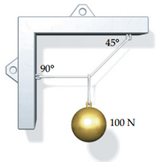
\includegraphics[width=0.5\textwidth]{75.png}
    \label{fig:75}
    \end{figure}
\subsection*{Hint 5}
Betrachten Sie das Kräftegleichgewicht am Knotenpunkt vektoriell. \\
Welches der beiden Seile kann die Gewichtskraft aufbringen? \\
Wie gross ist dann die gesamte Seilkraft? \\
Wer bringt die Horizontalkomponente auf?
\subsection*{Solution 5}
Die Kugel bewegt sich nicht, also müssen sich alle Kräfte aufheben.
Auf die Kugel wirkt die Schwerkraft nach unten von 100 N\\
Das schräge Seil muss deshalb vertikal 100 N aufbringen und in der Diagonalen $100 \sqrt{2} = 141$~N.\\
Horizontal zieht dann das schräge Seil mit ebenfalls 100 N nach rechts, was vom Seil mit 90° ausgeglichen werden muss. Es zieht mit 100 N nach links.
\subsection*{Question 6}
$\star\star$Die Trägheitsbewegung kann als Vergleichsbewegung herangezogen werden, um Rückschlüsse auf die Richtung real vorhandener Kräfte bei einer gegebenen Bewegung zu ziehen. Die real gegebene Bewegung sei die Kreisbewegung des Mondes um die Erde.\\
a) Gedankenexperiment: Wie würde sich der Mond im Verlaufe einer Zeitspanne bewegen, wenn die Erde augenblicklich verschwinden würde,\\
b) Wo befände sich der Mond bei Anwesenheit der Erde nach dieser Zeitspanne?\\
c) Welche Wirkung hat demzufolge die Erde auf den Mond, bzw. welche Richtung muss demzufolge die Kraft der Erde auf den Mond haben?\\
d) Verallgemeinern Sie: Wohin ist eine Kraft gerichtet, die einen Körper auf einer Kreisbahn hält?
\subsection*{Hint 6}
Es geht hier um die Richtung der Zentripetalbeschleunigung und -kraft.
\subsection*{Solution 6}
a) Der Mond fliegt tangential zur Kreisbewegung geradeaus (keine Kräfte – die Geschwindigkeit bleibt gleich, nach Betrag und Richtung).\\
b) Auf einer Kreisbahn – die Gravitation zwingt ihn dazu\\
c) Erde und Mond ziehen einander an, ganz grob kann man die Erde als fast in Ruhe annehmen und den Mond darum herum kreisen lassen. Wirklich kreisen beide um den gemeinsamen Schwerpunkt, der innerhalb der Erde liegt. \\
d) Sie ist auf das momentane Zentrum der Kreisbahn gerichtet, entlang dem momentanen Radius. Bei einer Kreisbahn ist das Zentrum immer am gleichen Ort, bei einem gekurvten Weg ändert sich der Ort des Zentrums.
\subsection*{Question 7}
$\star$Eine Kiste steht auf einem um einen Winkel $\alpha$ geneigten Hang und bewegt sich nicht.\\
Wählen Sie wie im Bild ein Koordinatensystem mit x parallel zum Hang und y senkrecht zum Hang\\
Zeichnen Sie Gewichts- und Normalkraft ein, die auf die Kiste wirken.\\
Berechnen Sie den Betrag der Normalkraft aus der Bedingung, dass die Kiste sich in y-Richtung nicht bewegt (sie sinkt nicht im Boden ein).\\
Berechnen Sie die vektorielle Summe von Gewichts- und Normalkraft
\begin{figure}[H]
    \centering
    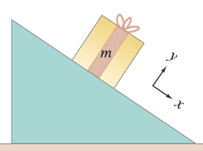
\includegraphics[width=0.5\textwidth]{77.png}
    \label{fig:77}
    \end{figure}
\[Bild: Giancoli, Physik\]
\subsection*{Hint 7}
siehe Folie Kräfte am Hang.
\subsection*{Solution 7}
Gewichtskraft senkrecht zum Blatt nach unten.\\
Normalkraft parallel zu y nach oben. Die Länge ist noch nicht bestimmt\\
Wir drücken die Gewichtskraft als Vektor im gewählten Koordinatensystem xy aus:\\
$\vec{F_G}=mg(sin\alpha,-cos\alpha)$. Die y-Komponente ist negativ, weil sie entgegen der y-Achse zeigt.\\
Die resultierende Kraft in y-Richtung ist $F_y=F_N-mgcos\alpha$ und muss 0 sein, weil sich der Körper in y-Richtung nicht bewegt.\\
Damit wird die Normalkraft $\vec{F_N}=(0,mgcos\alpha)$. Sie hat nur eine Komponente in y-Richtung.\\\\
\textbf{Vektorsumme}
Die resultierende Kraft ist die Vektorsumme
\[{\vec{F}}_{res}=\vec{F_G}+\vec{F_N}=mg(sin\alpha,-cos\alpha)+mg(0,cos\alpha)=mg(sin\alpha,0)\]
Diese Kraft zeigt in x-Richtung parallel zum Hang\\
In y-Richtung muss die Summe 0 geben, das haben wir in die Rechnung hineingesteckt, weil die Kiste sich senkrecht zum Boden nicht bewegt.
\subsection*{Question 8}
$\star\star$Ein Zug bestehe aus einer Lok und drei Waggons gleicher Masse $m=35$~t , die beim Anfahren mit 0.4 m/s$^2$ beschleunigt werden. Die Waggons werden mit A, B und C bezeichnet und sind als unterschiedliche Körper zu behandeln.\\
a) Fertigen Sie eine Skizze mit allen Kräften auf die einzelnen Waggons an.\\
b) Berechnen Sie die Zugkraft $F_Z$ der Lok und die Beträge der Kupplungskräfte $F_BA$ und $F_CB$.
\subsection*{Hint 8}
Welche Masse muss $F_Z$ beschleunigen, welche die anderen Kopplungskräfte?
\subsection*{Solution 8}
Skizze: A = B = C = Lok (das \guillemotleft = \guillemotright\ ist eine Kupplung)\\
Lok beschleunigt A+B+C mit $F_Z= a \cdot m  = 0.4 \cdot 3 \cdot 35'000 = 42$~kN\\
Wagen C beschleunigt noch Wagen A und B mit $FCB = 0.4 \cdot 2 \cdot 35'000 = 28$~kN etc.
\subsection*{Question 9}
$\star\star$Ein Tennisball wird mit einer Geschwindigkeit vom Betrage $v_0$ unter dem Winkel $\alpha$ gegenüber der Horizontalen abgeschlagen. Der Luftwiderstand wird vernachlässigt. Die y-Achse zeigt senkrecht nach oben.\\
a) Mit welcher Geschwindigkeit $v_x(t)$ bewegt er sich in horizontaler Richtung?\\
b) Mit welcher Geschwindigkeit $v_y(t)$ bewegt er sich in vertikaler Richtung?\\
c) Berechnen Sie die Zeitfunktion $r_x(t)$ für die Bewegung in horizontaler Richtung. \\
d) Berechnen Sie die Zeitfunktion $r_y(t)$ für die Bewegung in vertikaler Richtung.\\
e) Ermitteln Sie die Funktion $r_y(r_x)$ für die Bahnkurve des Tennisballs? Wie nennt man die spezielle Funktionskurve, die durch diese Funktion beschrieben wird?
\subsection*{Hint 9}
Stellen Sie allgemein die Bewegungsleichung in 2D auf (siehe Folien Schiefer Wurf). Damit können Sie a-d angeben.\\
Für e) ist eine Funktion für die y-Komponente des Orts gesucht, die nun nicht mehr von der Zeit abhängen soll, sondern von der x-Komponente. Dadurch wird die Bahnkurve beschrieben. Sie müssen dafür die Zeit eliminieren, z.B. indem Sie die Zeit in $r_y(t)$ durch einen Ausdruck mit $r_x(t)$ ersetzen.
\subsection*{Solution 9}
Es wirkt nur die Gravitationskraft, die Bewegungsgleichung ergibt sich deshalb wie meist in diesen Fällen zu:
\[\vec{v}(t)=\vec{a}t+\vec{v_0}\]
\[\vec{r}(t)=\frac{1}{2}\vec{a}t^2+\vec{v_0}t+\vec{r_0}\]
Wir setzen für $a$ und $v$ die Anfangsbedingungen ein:
\[\vec{v_0}=|\vec{v_0}|(\cos\alpha,\sin\alpha) \mathrm{,}a=(0,-g)\] \\
\[\vec{v}(t)=(0,-g)t+|\vec{v_0}|(\cos\alpha,\sin\alpha)\]
\[\vec{r}(t)=\frac{1}{2}(0,-g)t^2+|\vec{v_0}|(\cos\alpha,\sin\alpha)t+(0,0)\]\\
Damit sind die Fragen a-d beantwortet. a und b sind die Komponenten von $\vec{v}(t)$, c und d die Komponenten von $\vec{r}(t)$\\
Für die Frage e) müssen wir die Komponenten des Ortsvektors separat aufschreiben:
\[
r_x = |v_0| \cos \alpha t
\]
\[
r_y = -\frac{1}{2} g t^2 + |v_0| \sin \alpha t
\]
Wir lösen $r_x$ nach der Zeit $t$ auf und setzen in $r_y$ ein. Auf diese Weise eliminieren wir die Zeit $t$ und erhalten $r_y$ als Funktion von $r_x$:
\[
t = \frac{r_x}{|v_0| \cos \alpha} \quad (\cos \alpha \neq 0)
\]
\[
r_y = -\frac{1}{2} g \left( \frac{r_x^2}{(|v_0| \cos \alpha)^2} \right) + \frac{|v_0| \sin \alpha}{|v_0| \cos \alpha} r_x
\]
\[
r_y = -\frac{1}{2} g \left( \frac{r_x^2}{(|v_0| \cos \alpha)^2} \right) + \tan \alpha \, r_x
\]
Das sieht kompliziert aus, ist aber von der einfachen Form $y(x)=ax^2+bx.$ Das ist die Gleichung einer Parabel\\
Diese Form bezeichnet man auch als Wurfparabel.\\
Sie kommt zustande, weil sich der Körper horizontal mit konstanter Geschwindigkeit bewegt, vertikal aber konstant beschleunigt ist.
\end{document}



